%%%%%%%%%%%%%%%%%%%%%%%%%%%%%%%%%%%%%
%% Master Thesis - Computer Engineering
%% Copyright 2009 Ricardo Alexandre Fiorelli, Erick Poletto
%% This document is distributed by the terms of the license
%% included in the file LICENCE.
%%%%%%%%%%%%%%%%%%%%%%%%%%%%%%%%%%%%%

%%%%%%%%%%%%%%%%%%%%%%%%%%%%%%%%%%%%%
%% Third Chapter
%% Methodology
%%%%%%%%%%%%%%%%%%%%%%%%%%%%%%%%%%%%%

\chapter{Methodology} \label{chap3:methodology}

Write a review point of the problem and the solution I want to achieve\ldots

\section{Overview} \label{sec3:overview}
    This research was conducted in order to determine how much energy a computer's components, for instance, CPU, Memory and Hard Drives spend and, also, how much it would affect the cost of the Data Center in a whole. Above that, the advantages and disadvantages as well as the reliability of these measures and benchmarks played also an important role in the objectives of this thesis work. With regard to the topic in hand, the analysis was carried on with the help of Softwares, which will be explained in the following sections and analytical measures using an energy measurement device to counterbalance and compare the benchmarking measures obtained from these softwares. Concretely, more than 1000 components were analyzed and categorized in a huge database, which the schema can be seen on Figure~\ref{fig:database_schema}. Firstly, it was used the Sandra's database~\ref{sec3:sandra} to collect the components and separate them by categories, with their benchmarks and all data. Secondly, it was used WebSPHINX~\ref{sec3:websphinx} for the collection of components and linkage of MPN\footnote{Manufacturer Part Number} and the respective component. Thirdly, it was used an analytical method using a energy measurement device~\ref{sec3:energy_measurement_instrument} for the comparison and validation of the results given by the other benchmarks. 

    Finally, these data were all linked in a database for later comparison and choice. 

\section{Research Design} \label{sec3:research_design}
    % TODO

\section{Energy Management and Benchmarking Tools} \label{sec3:energy_management_tools}
    In order to obtain relevant information about the data required for making the comparison between the components, it was needed to use some energy management and benchmarking tools. 
    
    The softwares used, were selected from many of existents softwares in the area for the following reasons:
\begin{description}
	\item[Size of Database] The database of components, in order to get a good result should be considerably big;
	\item[Characteristics of Benchmarks] The benchmarks provided by the software should provide information about the energy consumed for each component;
	\item[Number of Benchmarks] The software should have a good database of benchmarks;
	\item[Quality of Benchmarks] Although, the number of benchmarks should be sufficiently, the quality, precision and relevancy were, also, important in the decision method;
	\item[Ease of Use] In the sense that, the software should provide an ambient of work that is intuitively and comfortable;
	\item[something1] explain ;% TODO
	\item[something2] explain ;% TODO
	\item[something3] explain ;% TODO
\end{description}
    
    The acquisition of data was made analyzing the results of these benchmarks, making use of their database

\subsection{SiSoftware SANDRA} \label{sec3:sandra}

    SiSoftware Sandra\footnote{The \textbf{S}ystem \textbf{AN}alyser, \textbf{D}iagnostic and \textbf{R}eporting \textbf{A}ssistant} is an information and diagnostic utility. It provides most of the information (including undocumented) one need to know about their hardware, software and other devices whether hardware or software.
SANDRA was the main software utilized to benchmark the data in this thesis work. It contains a huge database of components to make sure the benchmarks provided have the best results and accurate comparisons.
    
    The software goes beyond the point of other Windows Utilities, by giving the user, the possibility of benchmarking and comparing at both high and low level the computer devices. Moreover, it is a tool for monitoring the performance on systems and even benchmarking many parts of the computer, this includes, CPU\footnote{Central Processing Unit}, memory, hard disks, CD/DVD ROM, network, PSU\footnote{Power Supply Unit}, etc. For that reason, it is considered one of the most complete benchmarking tools available. Besides the benchmarking, Sandra also provides access to information about the Hardware, including the Motherboard, processor, disks, printers, etc; and Software, such as, key softwares (web browsers, e-mail program, etc.), OS information, processes, memory usage and more.
    
    The detailed list of modules utilized by SiSoftware Sandra can be found in Appendix~\ref{app:sandra_modules}.
    
    Furthermore, the Sandra has a great functionality that is a catalog of pricing, which, in addition to the power consumption and other important characteristics, the best combination (which means the most green) of devices can be chosen to the server.
    
\subsection{Energy Measurement Instrument} \label{sec3:energy_measurement_instrument}

    \begin{figure}[!htb]
        \centering
            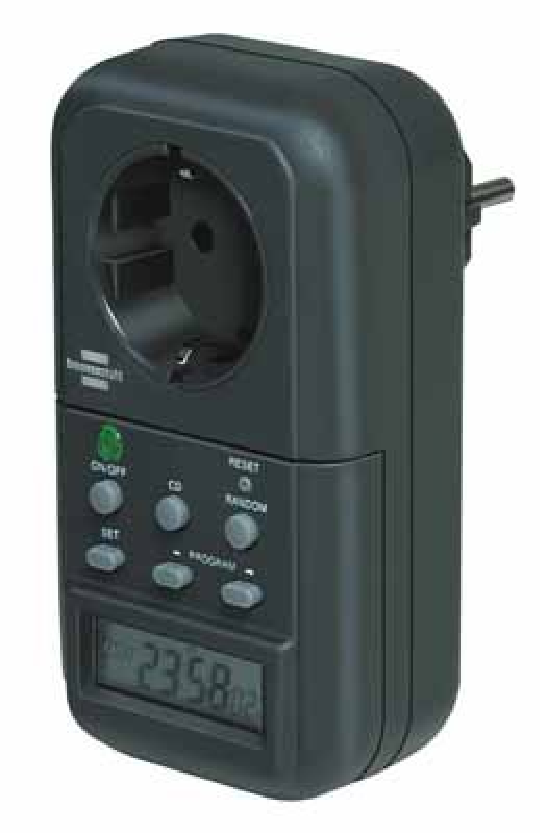
\includegraphics[scale=0.6]{graphics/energy_measurement_instrument}
            \caption{Energy Measurement Instrument}
            \label{fig:energy_measurement_instrument}
    \end{figure}
The device, which can be seen on Figure~\ref{fig:energy_measurement_instrument}, was used for comparing and validating with the results of the benchmarks given by Sandra.

After the result of the benchmark was obtained from the SiSoftware Sandra, this equipment that was connected to the computer read how much energy it was consumed and it was inserted in the database.
    % TODO
\subsection{WebSPHINX - A Personal, Customized Web Crawler} \label{sec3:websphinx}
    WebSPHINX\footnote{Website-Specific Processors for HTML Information Extraction} is a Java class library used for web crawling. It provides a way to browse and process web pages automatically.
    
    This piece of software was used to establish the pricing, linking it with the MPN\footnote{Manufacturer's Part Number}, and, afterwards, composing the database explained in \ref{sec4:analysis}. 
    % TODO
\subsection{CPU-Z} \label{sec3:cpu-z}
    CPU-Z detects information about the CPU, RAM Memory, motherboard, chipset and more. That program was used to complete the database with missing information about the components.
    % TODO
\subsection{PlateSpin - Recon} \label{sec3:power_recon}
    This software did not compose the ones used for doing this thesis. Yet, it is important to notice this, because it is almost the same of Sandra, but it provides a more incisive work on Data Centers in general. It provides workload profiling, analysis and planning of complex server consolidation, disaster recovery, capacity planning, asset management and green data center initiatives. It also provides forecasting for optimizing the data center by collecting hardware, software and services inventory for all server workloads. Furthermore, it results an statistics work for the server workloads running on data center and how their resources are being used.
    
    For the reason that it was needed to compare the components, in order to draw a picture of the most suitable components to be used. It was chosen Sandra, which has a great database of components.

\section{Data Processing and Analysis} \label{sec3:data_processing_analysis}
    % TODO
